\documentclass[11pt]{article}       % The percent symbol in your code starts a comment.  The comment ends at the next linebreak.
\usepackage[english]{babel}         % Packages add functionality and style conventions to your documents. Don't edit this section!
\usepackage{fullpage}               % Eliminates wasted space
\usepackage[utf8]{inputenc}         % Necessary for character encoding
\usepackage{amsmath, amssymb,amsthm}% Required math packages
\usepackage{graphicx}               % For handling graphics
\usepackage[colorinlistoftodos]{todonotes}  % For the fancy "todo" stuff
\usepackage{hyperref}               % For clickable links in the final PDF
\usepackage{tikz}
\theoremstyle{definition}
\newtheorem{theorem}{Theorem}
\newtheorem{lemma}[theorem]{Lemma}
\newtheorem{prop}[theorem]{Proposition}
\newtheorem{claim}[theorem]{Claim}

\title{Complex Analysis -- Homework \#7}

\author{ Komissar, Feldman, Kallus }

\date{ Due Friday, February 19 }

\begin{document}
\pagecolor{black}
\color{white}
\maketitle

\noindent{\bf 1. Exercise 11.7 }  Show that if $c \ne 1$ is an $n$-th root of unity, then $$1 + c + c^2 + \cdots c^{n-1} = 0.$$
\begin{proof}
To begin, for any $z \in \mathbb C$ and any $n \in \mathbb N$, the distributive property gives
\begin{align}
(1 + z + z^2 + \cdots z^{n-1})(1-z) &= (1 + z + z^2 + \cdots z^{n-1})-z(1 + z + z^2 + \cdots z^{n-1}) \\
&= 1 + z + z^2 + \cdots z^{n-1} - z - z^2 - z^3 - \cdots - z^n \\
&= 1 + z + z^2 + \cdots z^{n-1} - z - z^2 - z^3 - \cdots - 1 \\
&= 1 + z + z^2 + \cdots z^{n-1} - 1 - z - z^2 - z^3 - \cdots - z^{n-1} \\
&= 1 - z^n.
\end{align}
Thus, if $c \ne 1$ is an $n$-th root of unity, then $$(1 + c + c^2 + \cdots c^{n-1})(1-z) = 1 - c^n = 1 - 1 = 0.$$
Thus, either $1 + c + c^2 + \cdots c^{n-1} = 0$ or $1 - c = 0$.
Since $c \neq 0$, it must be that $$1 + c + c^2 + \cdots c^{n-1} = 0.$$
\end{proof}

\vskip.1in
\hrule
\vskip.1in

\newpage{\bf 2. }  Let $f(x)=\dfrac{1}{1-x+3x^2}$.
\vskip.05in
\noindent {\bf a. } Find the real polynomial $p(x) = p_0 + p_1x + p_2x^2 +p_3x^3$  that agrees with $f$ at the equally-spaced points $x_0=-1$, $x_1=-1/3$, $x_2=1/3$, and $x_1=1$; this is the \emph{cubic interpolant of $f$} for the given points. Indicate the set-up for your approach, but you need not include every step of the derivation. You may employ technology to perform computations.

We are looking for values of $p_0, p_1, p_2, p_3$ such that $p(-1) = \frac15$, $p\left(-\frac13\right) = \frac35$, $p\left(\frac13\right) = 1$, and $p(1) = \frac13$.

Thus, we need to solve the following system of equations:
\begin{align*}
    p_0 + p_1 + p_2 + p_3 &= \frac13 \\
    p_0 - P_1 + p_2 - p_3 &= \frac15 \\
    p_0 + \frac13p_1 + \frac19p_2 + \frac1{27}p_3 &= 1 \\
    p_0 - \frac13p_1 + \frac19p_2 - \frac1{27}p_3 &= \frac35
\end{align*}
The solution to this system is $$p_0 = \frac{13}{15}, ~~~ p_1 = \frac23, ~~~ p_2 = -\frac35, ~~~ p_3 = -\frac35.$$

Thus, $$p = \frac{13}{15} + \frac23x - \frac35x^2 - \frac35x^3.$$

\noindent
\dotfill

\newpage {\bf b. } On the same set of coordinate axes, provide a computer-generated graph of both $f$ and $p$ on the interval $[-1,1]$.

$f$ is shown in teal, and $p$ is shown in magenta in the graph below:
\begin{center}
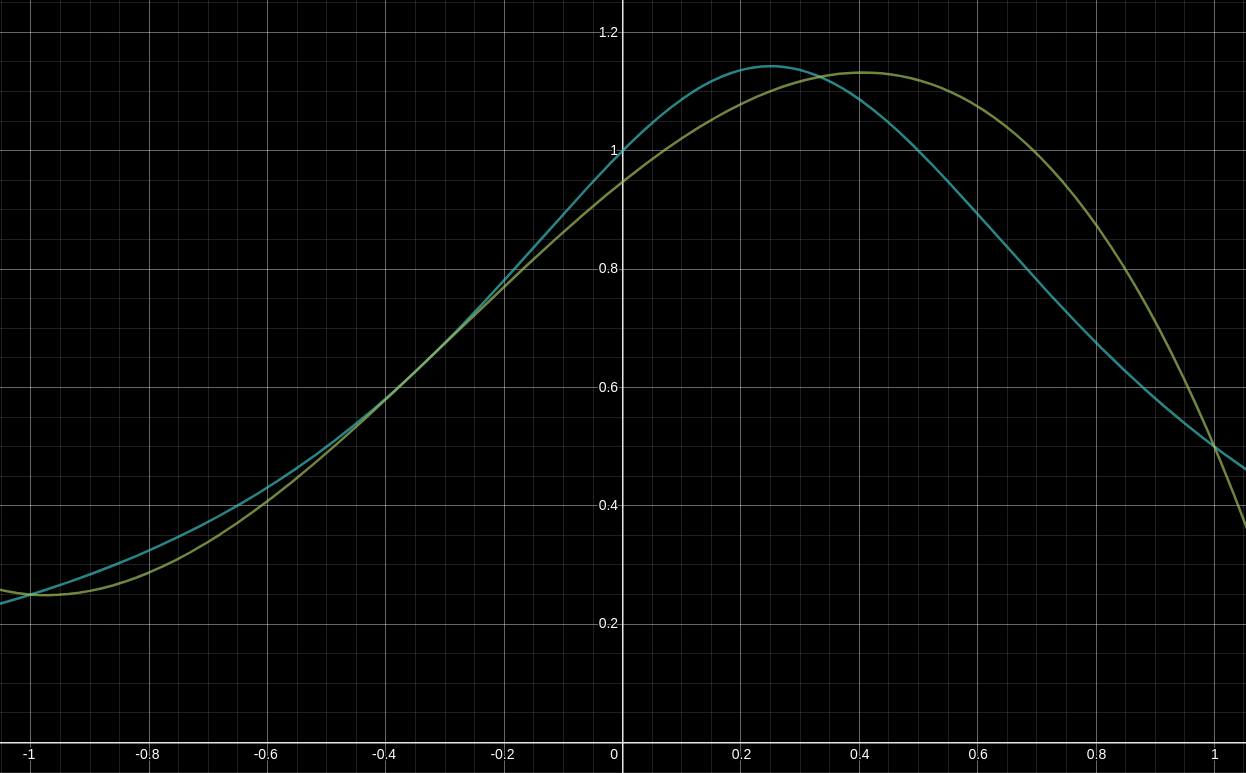
\includegraphics[scale=.75]{07.png}
\end{center}

\vskip.1in
\hrule

\end{document}